In this chapter we are looking at the basics of how sourdough ferments.
For that we will first look at enzymatic reactions
that happen in your flour. These reactions are induced
the moment you add water to your flour. They are also
the basis that trigger the fermentation process. To understand
the fermentation process we are having a closer look at the involved
yeast and bacterial microorganisms.

\begin{figure}[!htb]
  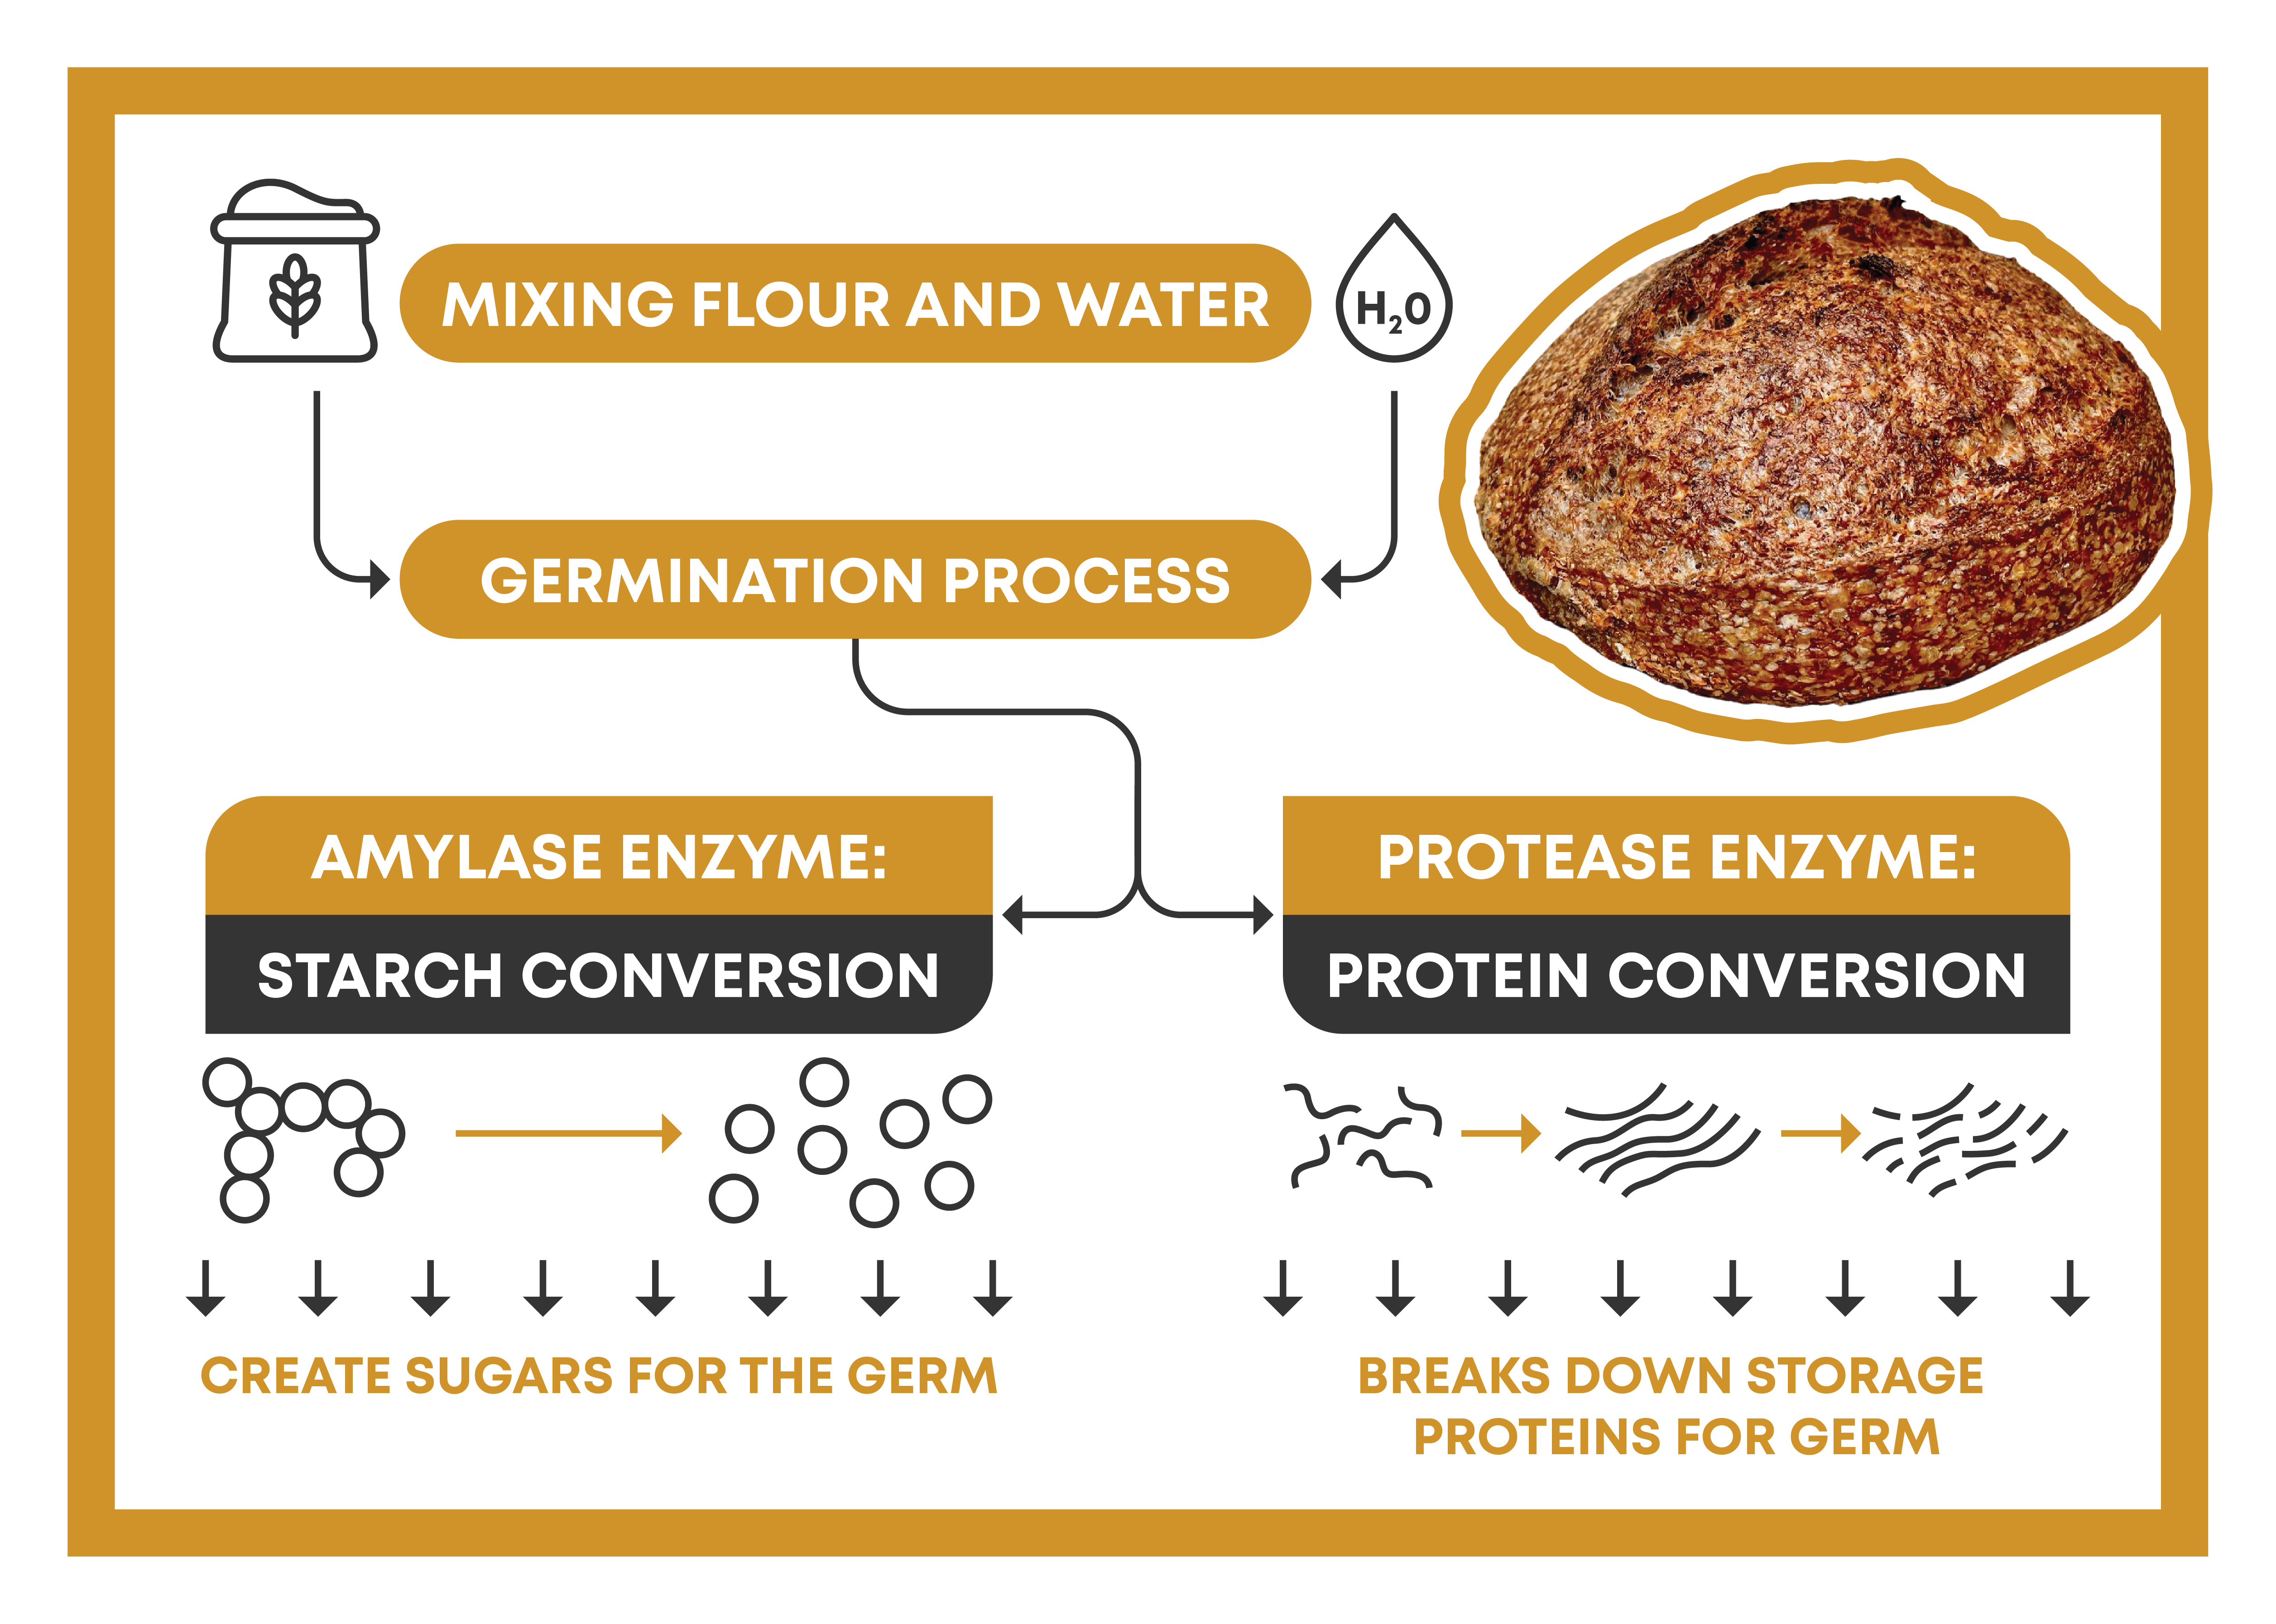
\includegraphics[width=\textwidth]{infographic-enzymes}
  \caption{How amylases and proteases interact with flour}
  \label{infographic-enzymes}
\end{figure}

\section{Enzymatic reactions}

When mixing flour and water several enzymatic reactions
start. A plant produces seeds to reproduce. The seed
contains all the nutrients a new plant needs to sprout.
While the seed is dry the seed is in hibernation mode. It
can be sometimes be stored for several years. The moment water is added
to the seed the sprouting process starts. The seed turns
into a germ. The stored nutrients have to be converted
into something that the germ can use. The catalyst for these
reactions is water. The first roots can be produced with the stored nutrients.
Furthermore the seed typically contains the first leaves
of the plant. The first leaves are built to start the photosynthesis
process. This is the plants' engine. With energy from photosynthesis
the plant can keep growing more roots. This way more water
and nutrients can be accessed from the soil. The extended 
nutrients allow the plant to form more leaves and thus
increase the photosynthetic activity.

Of course a ground flour can no longer sprout. But the enzymes
that trigger this process are still present. That's why it's
important to not mill the grains at a too high temperature.
This could possibly damage some of the enzymes. Normally
the seed of the flour shields the germ against pathogens initially.
However as we grind the flour the contents of the seed
are exposed. This is ideal for our sourdough microorganisms.
The yeast can be considered a saprotrophic fungus.
They can't prepare their own food. As the enzymes start
to be activated more and more food becomes available
for the yeast and bacteria.

The two main enzymes for bread making are amylase and protease.
Understanding their role is a key puzzle piece to be able
to make better tasting bread at home.

\subsection{Amylase}

Sometimes when you chew on a potato or a piece of bread
for a prolonged period of time you will notice a bit of sweetness
arising in your mouth. That's because your salivary glands
are also producing amylase. Amylase breaks down complex
starch molecules into easier digestible sugars. The germ
needs this in order to be able to produce more plant matter.
Your body needs this in order to start the digesting process.
Normally your microorganisms can't consume the freed maltose molecules
as they are hidden in the germ. But as we ground the flour
a feeding frenzy starts. Generally the warmer the temperature
the faster this reaction happens. That's why a long fermentation
is a key factor to make great bread. It takes time
for your amylase to break down most of the starch. Furthermore
not all sugars are consumed by the yeast. Some remain and
are responsible for enhanced browning during the baking
process.

If you are a hobby brewer you will know that it's
important to keep your brew on certain temperatures for a
while to allow the different amylases to convert starches
into sugar \cite{beer+amylase}. There's a test frequently used by brewers
to determine that all the starches have been converted.
It's called the Iodine starch test. You take a bit of your brew
and then add a bit of iodine. If the color is blue/black
you know that you still have starches left that haven't been
converted by amylases yet. I wonder if such a test would work
for a bread dough as well? Now industrial bakeries
that use yeast to make speed doughs in a short period of
time face this issue. Their approach is to add malted
flour to the dough mix. The malted flour contains a lot
of enzymes and will thus help to have a faster fermentation
period. Check the packaging of the breads that you bought,
if you find {\it malt} in the list of ingredients chances
are that this strategy has been used. There are two categories
of malts. You have enzymatically active malt and inactive
malt. The active malt hasn't been heated to above 70°C
when the amylases start to degrade under heat. The inactive
malt has been heated to higher temperatures and thus
has no impact on your flour.

\subsection{Protease}

The second very important enzyme is the protease. Proteases
break down proteins into smaller proteins or amino acids.
Gluten for instance is a storage protein built by wheat.
The gluten is broken down and converted the moment the
seed starts to sprout. That's because the seed needs
smaller amino acids to build the roots and other plant material.
If you ever try to make a wheat based dough and just keep
it for several days at room temperature you will notice
how your gluten network starts to break down. The dough
no longer holds together. You can just fully tear it apart.
I have had this happen to me when I was trying to make
doughs directly with dried sourdough starter. The fermentation
speed was so low that it took 3-4 days for the dough
to be ready. The root cause for this issue is the protease.
By adding water to the dough the protease was activated
and started to ready amino acids for the germ in order to be
able to sprout. Another interesting experiment that viusalises
the importance of protease is the following. Try to make a
fast dough within 1-2 hours. Simply use a large quantity
of dry yeast. Your dough will be leavened and increase in size.
Bake your dough and notice the crumb of your baked dough.
You will notice that the crumb is quite dense and not as
fluffy as it could be. That's because the protease enzyme
didn't have enough time to do its job. At the start
when kneading your dough is very elastic. It holds together
very well. Over the course of the fermentation process
your dough will become more extensible \cite{protease+enzyme+bread}.
Some of the gluten bonds start to naturally break
down due to the protease proteolysis. This makes it easier
for your dough to be inflated. That's why a long
fermentation process is important when you want to
achieve very fluffy and open crumbs with your sourdough
bread. Next to using great ingredients, the long and
slow fermentation is one of the main reasons why
Neapolitan pizza tastes so great. The soft and fluffy
edge of the pizza is achieved because of the protease
creating a very extensible easy to inflate dough. Because
the fermentation process is typically longer than 8
hours a flour with a higher gluten content is used. There
is more gluten that can be broken down by the protease.
By using a weaker flour you might end up with a dough
that's already broken down too much and will then tear
when trying to make a pizza pie. Traditionally the pizza
has probably been made with sourdough. In modern times
it is made with yeast as handling a yeast based
dough can be done easier on a larger scale. The dough
stays good for a longer period of time. If you were to use
sourdough you might have a window of 30-90 minutes when
your dough is perfect. Afterwards the dough might
start to deteriorate because of bacteria breaking
down the gluten network too much.

\subsection{Improving enzymatic activity}

As explained previously malt is a common trick used
to speed up enzymatic activity. I personally prefer
to avoid malt in most of my recipes. Instead I use
a trick I observed when making whole wheat doughs.
No matter what I tried I could never achieve baking
a whole wheat bread with the desired crust and crumb
texture I was looking for. My doughs would tend to
overferment relatively quickly. When using a flower
with a similar amount of gluten that didn't contain
bran and other outer parts of the grain my doughs turned
out great. I was utilizing an extended autolyse.
That's a fancy word for just mixing flour and water in
advance and letting that mixture sit. Most recipes
call for it as the help to make a dough that has already
started to break down by enzymes. In general it's a great
idea but at the same time you can just reduce the amount
of leavening agent you use. This way the same biochemical
reactions happen and you don't have to mix your dough
several times. My whole wheat game drastically improved
when I stopped using the autolysis. It makes sense if I
think about it now. The first parts of the seed that
are in contact with water are the outer parts. Water
will slowly enter the center parts of the grain. The
moment the seed starts to sprout it needs to outcompete
other nearby seeds. Furthermore it also directly becomes
exposed to other animals and potential hazardous bacteria
and fungi. To accelerate this process most of the enzymes
of the grain are in the outer parts of the hull. They
are being activated first (source needed). So by just
adding a little bit of whole flour to your dough you 
will improve enzymatic activity of your dough. That's
why most of my plain flour doughs typically contain
at least 10-20 percent whole wheat flour.

\begin{figure}
  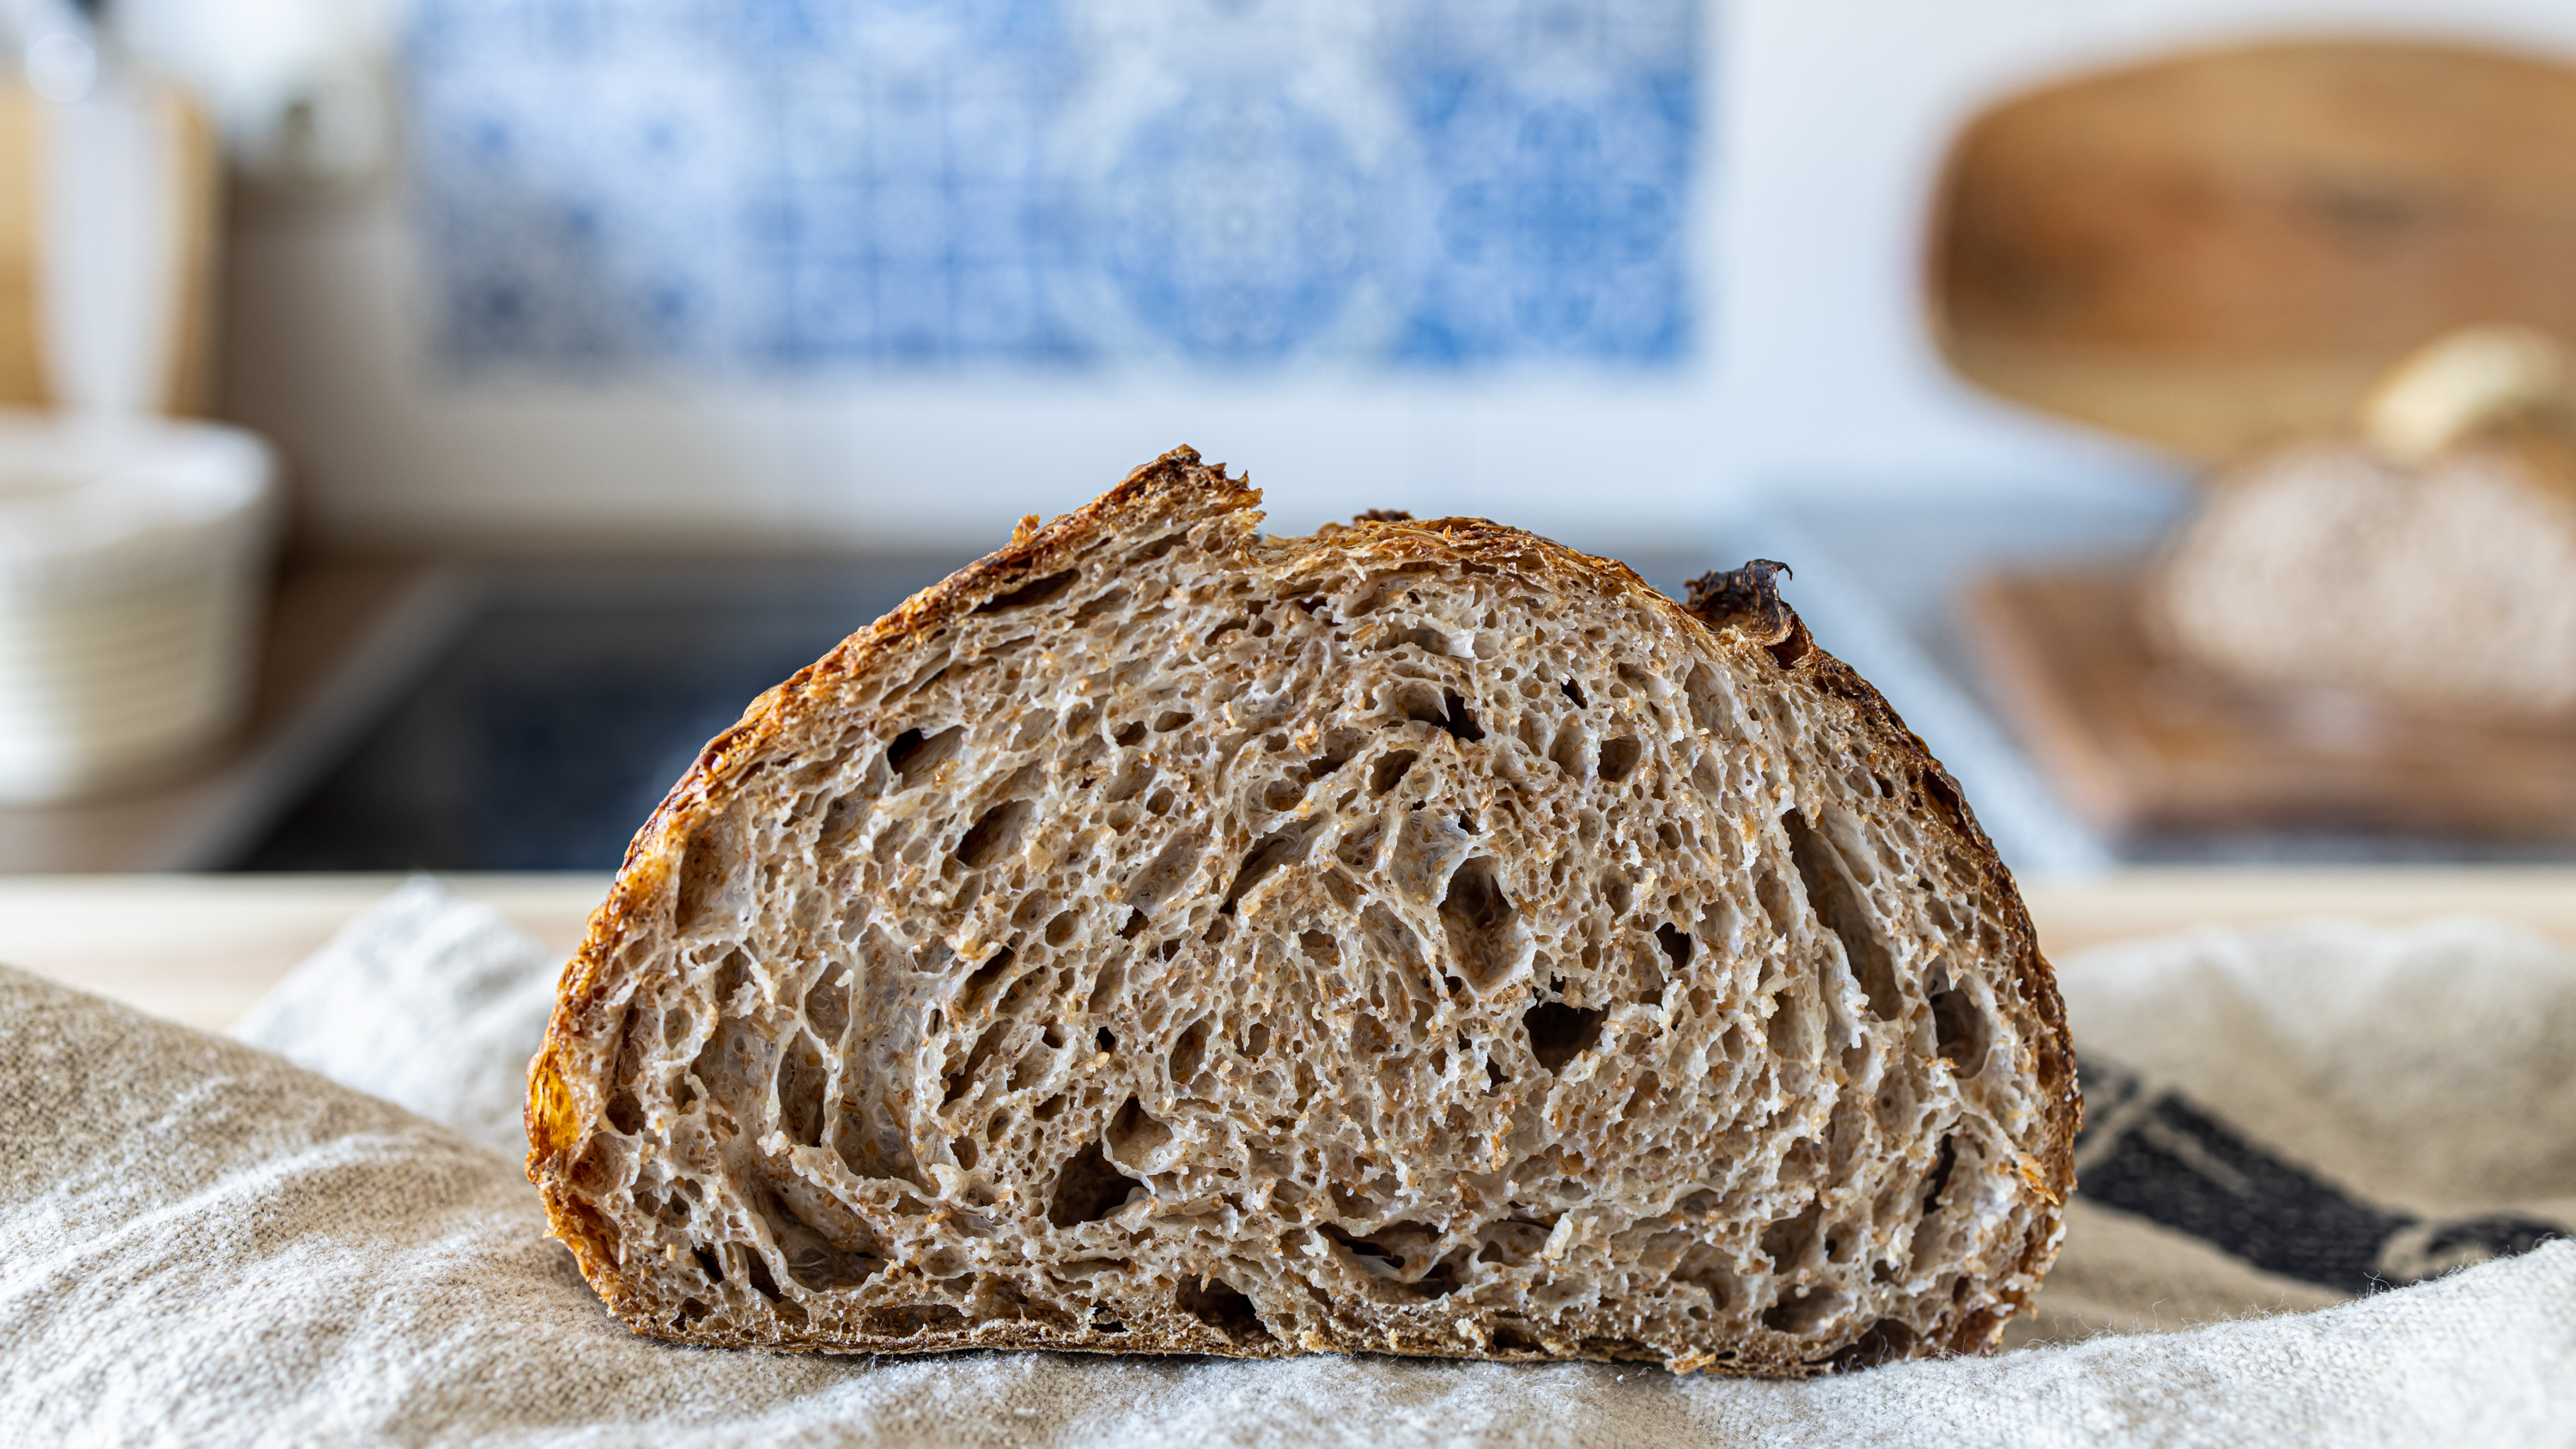
\includegraphics[width=\textwidth]{whole-wheat-crumb}
  \caption{A whole wheat sourdough bread}
  \label{whole-wheat-crumb}
\end{figure}


By understanding the 2 key enzymes amylase and protease
you will better be able to understand how to make a
dough to your liking. Would you like a dough a softer
or stiffer crumb? Would you like to achieve a darker crust?
Would you like to reduce the amount of gluten in your
final bread? These are all factors you can influence
by adjusting the speed of fermentation.

\section{Yeast}

Yeasts are single celled microorganisms that are part of
the fungus kingdom. Yeast spores that are hundreds
of million years old have been identified by scientists.
There is a wide variety of species and so far around 1500
different species have been recognized. Yeasts are not creating
a mycelium network like mold does for instance
\cite{molecular+mechanisms+yeast}.

\begin{figure}[!htb]
  \centering
  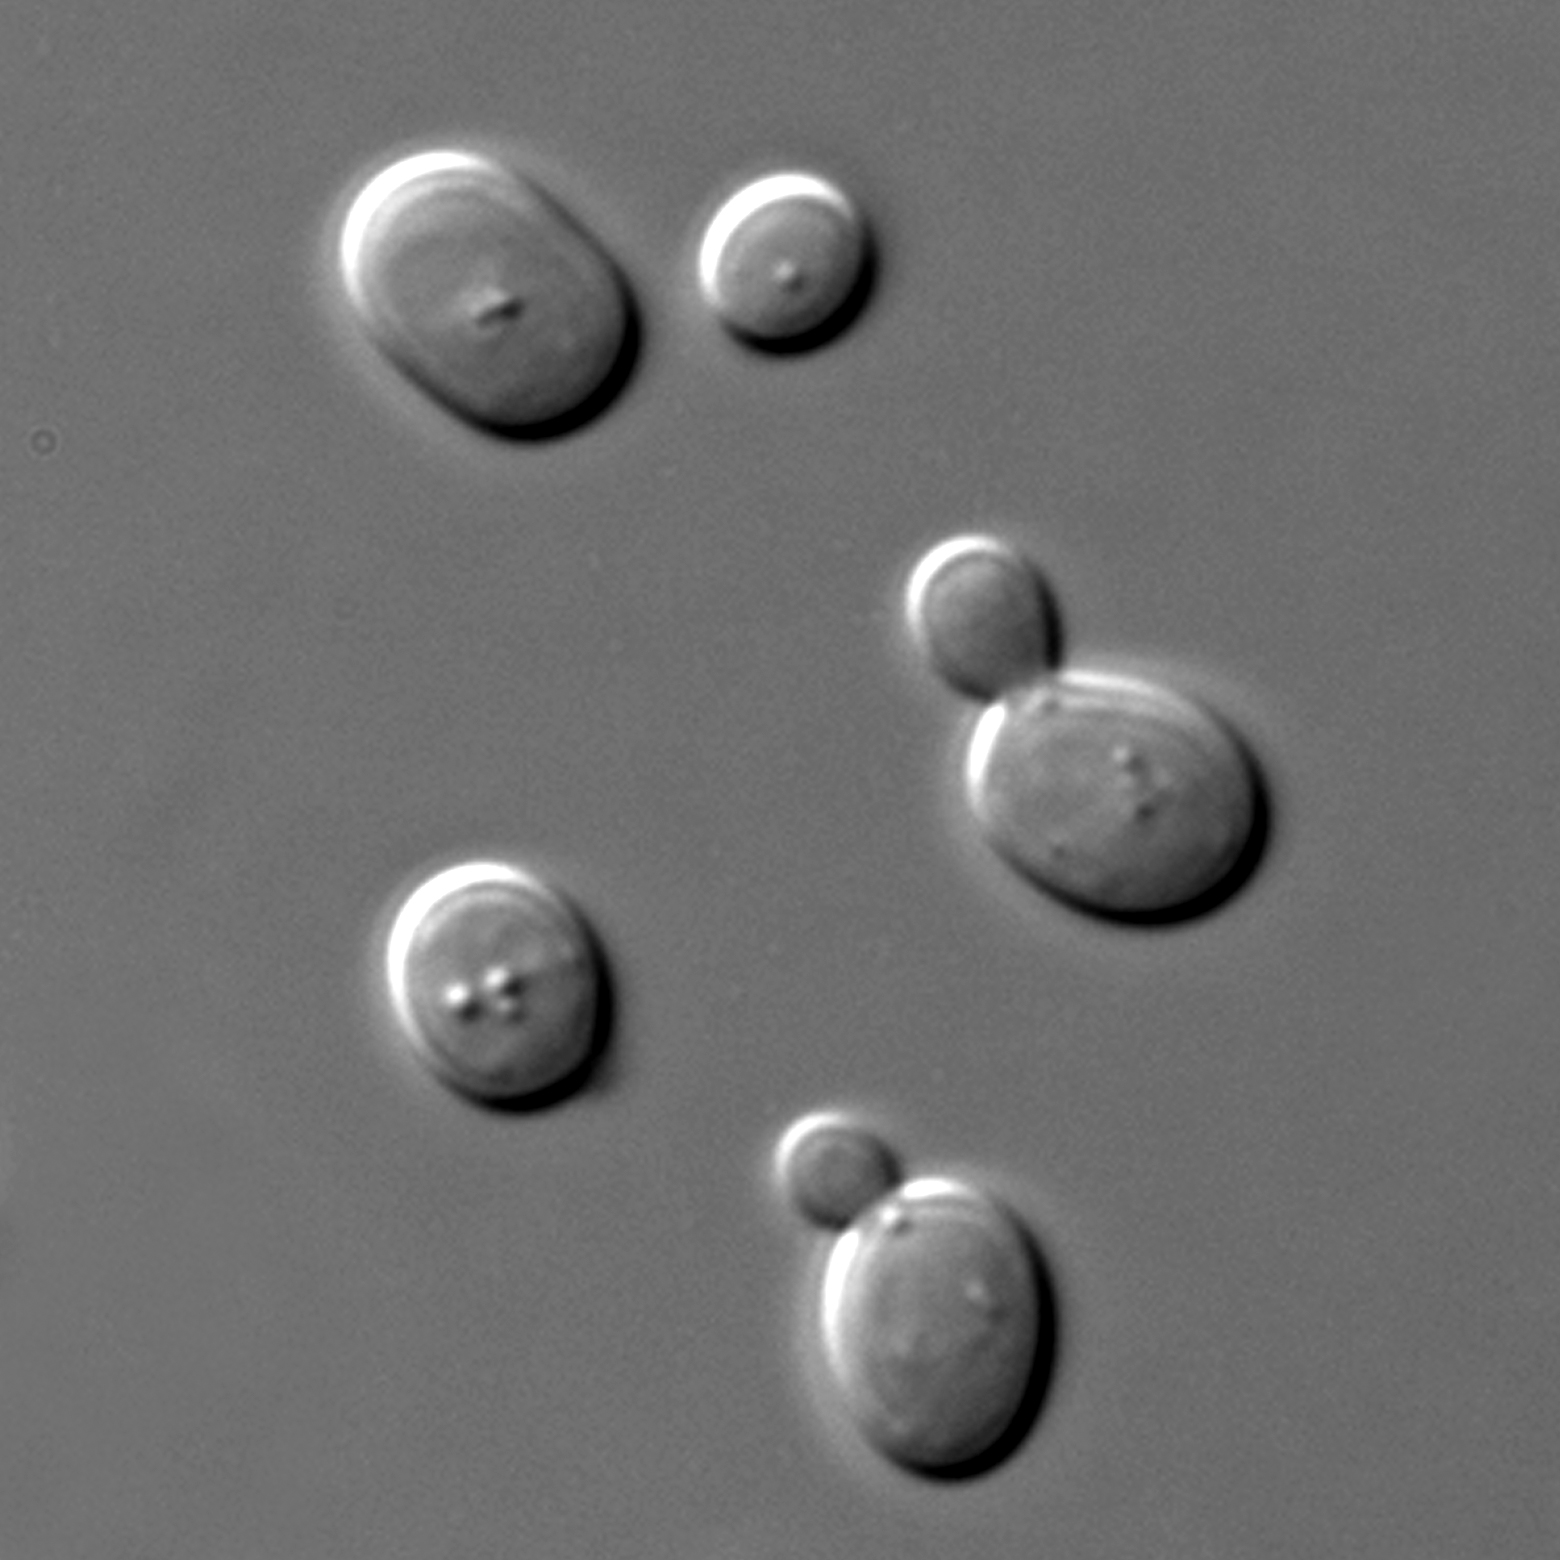
\includegraphics[width=1.0\textwidth]{saccharomyces-cerevisiae-microscope}
  \caption{Saccharomyces cerevisiae: Brewer's yeast under the microscope}
  \label{saccharomyces-cerevisiae-microscope}
\end{figure}


Yeasts are saprotrophic fungi. This means they are not
producing their own food. They rely on external food sources
which they decompose and break down. For yeasts
carbohydrates and broken down to carbon dioxide and
alcohols. The products of this fermentation process
have been used for thousands of years when making
bread or alcoholic beverages. Yeasts can grow
in both aerobic and anaerobic conditions. When oxygen
is present the yeast almost completely produces
carbon dioxide and water. When no oxygen is present
the yeast starts switches its metabolism. The
yeast starts to produce alcoholic compounds \cite{effects+oxygen+yeast+growth}.
The temperatures at which the yeast grows vary. Some
yeasts such as {\it Leucosporidium frigidum} grows
best at temperatures between -2°C up to 20°C. Other
yeast grows better at higher temperatures. The warmer
it is the faster the yeast's metabolism works. The yeast
that you cultivate in your sourdough starter works best
at the temperatures where the grain was grown and at
the point when it was harvested. So if you are from a 
cooler place and cultivate a sourdough starter from
a nordic rye variety, then chances are your yeast
prefers this colder environment. As an example
beer makers discovered that a beneficial yeast lives
in the cold caves around the city of Pilsen, Czech Republic.
This yeast has produced excellent tasting beers at
lower temperatures. Varieties of these strains
are now used to make popular lager beers.

Yeasts in general are very common in the environment.
They can be found on cereal grains, fruits, other plants
in the soil and also in your gut. Very little is known
about the ecology of why yeasts we use for baking
are cultivating the leaves of the plants. The plants
are protected via the cell walls and hardly any
fungi and other bacteria can penetrate. Some fungi and
bacteria are producing enzymes that are able
to break down the cell walls and infect the plant.
There are fungi and bacteria that live within the plant
without causing any distress. These are known as {\it endophytes}.
They are not damaging the plant per se. In fact they are
living in a symbiotic relationship with the host. They
help the plant to protect itself from additional pathogens
that might enter through the leaves of the plant. They
help with water stress, heat stress and nutrient availability. 
In exchange for the service they receive carbon for energy
from the plant host. They are not always strictly mutualistic though.
Sometimes under stress conditions they can become pathogens
on their own \cite{endophytes+in+plants} and decay begin
decaying the plant.

The yeasts we use for baking are
living as as epiphytes on the plant. Compared to
the previously mentioned endophytes they are not
breaching the walls of the cells. Most of them
receive nutrients from rain water, the air or other animals.
These sources also include honeydew produced
by aphids. Pollen that lands on the leaf's surface
is an additional source of food. Interestingly
though when you remove that external food source,
you still find a large variety of epiphytic fungi
and bacteria on the plant's surface. The food
for them is coming directly from the plant it seems.
Some research has shown that the plants are
on purpose releasing some compounds such as sugars,
organic acids, amino acids, some methanol and various
salts via the surface. These nutrients would
then attract the epiphytes to live on the surface.
The plants benefit from enhanced protection against
mold and other pathogens. It is in the best interest
of the epiphytes to keep the plants alive
as long as possible \cite{leaf+surface+sugars+epiphytes}.
More and more research is conducted on using yeasts
as a biocontrol agents to protect plants. These bio-agents
would be food-safe as yeasts are generally considered save.
The yeasts would start to grow on the leaves on the plant
and essentially shield the plants from other molds. This
could be a game changer for wineyeards suffering from mildew.
This could also be helpful to shield the plant against the
psychoactive ergot fungus. The ergot fungus likes to grow
in more humid colder environments and poses a huge
problem to rye farmers. The fungus parasites the plant
and infects it. Consumption of ergot is not recommended
as it is highly toxic to the liver. That's why lawmakers
have recently reduced the amount of allowed ergot contamination
in rye flour. Another interesting experiment from Italian scientists
visualized how important yeasts could be when protecting
plants. They added tiny incisions into some of the grapes.
They would then infect some of the damaged surfaces with
mold. The other wounds they infected with some of the 150
different wild yeast strains isolated from the leaves plus
the mold. When mixing the mold with the yeast the grape
sustained no significant damage \cite{yeasts+biocontrol+agent}.
In another experiment however scientists have shown
how the brewer's yeast became an aggressive pathogen to wine plants.
Initially the yeast lived in symbiosis with the plant. After the grapevine
sustained damages the yeast became opportunistic and started to
attack the plant event producing hyphae to deeply
penetrate the plants tissue.

\section{Bacteria}